\section{Durchführung und Messung}
\subsection{Durchführung}
In diesem Versuch wird für die Messung ein D8-Diffraktometer der Firma Bruker-AXS verwendet. In diesem
ist zum Erzeugen der Röntgenstrahlung eine Röntgenröhre mit Kupferanode verbaut,
welche mit einem Strom von $\SI{35}{\mA}$ und einer Spannung von $\SI{40}{\kV}$ betrieben wird.
Sowohl die Röntgenröhre als auch der Detektor sind um den Probentisch drehbar, um eine optimale Justage zu ermöglichen.

Da die aus der Röntgenröhre austretende Strahlung divergent ist, wird diese mit einem sogenannten Göbel-Spiegel
gebündelt und monochromatisiert, wodurch ein paralleler Strahl mit einer Wellenlänge von $\lambda=\SI{1,54}{\angstrom}$
erzeugt wird, welche der Kupfer $K_{\alpha}$-Linie entspricht. Ein Göbel-Spiegel besteht aus mehreren parabolisch gekrümmten Schichten,
wodurch sich nach Reflexion der divergenten Strahlung ein paralleler Strahl ergibt.

Bevor die Strahlung auf die Probe fällt, passiert sie einen Autoabsorber und eine Blende, um Streustrahlung zu minimieren.
Der Strahl durchläuft eine weitere Blende, nachdem er an der Probenoberfläche reflektiert wurde, um auch die Streustrahlung
nach der Reflexion zu reduzieren. Der schematische Aufbau aus Röntgenröhre, Probe und Detektor ist in Abbildung
\ref{fig:aufbau} dargestellt.

\begin{figure}
  \centering
  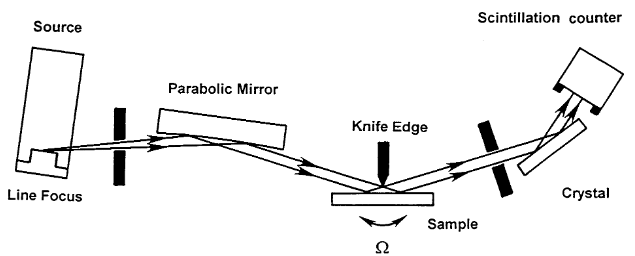
\includegraphics[width=10cm]{aufbau.png}
  \caption{Aufbau aus Röntgenröhre, Probe und Detektor \cite{aufbau}.}
  \label{fig:aufbau}
\end{figure}

Bevor mit der eigentlichen Messung begonnen werden kann, muss das Gerät justiert werden. Dazu stehen drei Scan-Methoden zur Verfügung:
\\
\textbf{1) Detektor-Scan}\\
Um den Detektor-Scan durchführen zu können muss die Probe zunächst aus dem Strahl herausgefahren werden. Bei dem eigentlichen
Detktor-Scan wird sowohl die Röntgenröhre, als auch der Detektor auf die Position $\SI{0}{\degree}$ gefahren. Um die tatsächliche Null-Lage des
Primärstrahls zu bestimmen, wird nun die Detektorposition um kleine Winkel variiert und so das Maximum des Primärstrahls ermittelt, welches
einer Gaußverteilung entsprechen sollte. Die Position des Maximums wird als neue Nullposition des Detektors verwendet.


\textbf{2) Z-Scan}\\
Da bei einer idealen Justage der Strahl parallel zu Probenoberfläche stehen sollte und die Probe die halbe Intensität des Primärstrahls abschotten solle,
wird als zweiter Schritt der Z-Scan durchgeführt. Wie der Name schon sagt, wird bei diesem Scan die z-Position der Probe verändert, indem sie langsam in den
Strahlengang gefahren wird, bis die gemessene Intensität von $I_{max}$ bis auf $\frac{1}{2}I_{max}$ abgenommen hat.
\\

\textbf{3) Rocking-Scan}\\
Bei dieser Scan-Methode werden die Röhre und der Detektor so um die Probe gedreht, dass die Winkelsumme $\alpha_i + \alpha_f=2\theta$ konstant bleibt, dies entspricht
einer Drehung der Probe. Durch diesen Scan können Informationen über die Verkippung der Probe im Strahl gewonnen werden. Ist die Probe gut positioniert liefert dieser
Scan einen dreieckigen Kurvenverlauf.
\\

Der Detektor-Scan wird zu Beginn der Justage nur einmalig durchgeführt, anschließend werden der Z-Scan und der Rocking-Scan mehrfach wiederholt, bis das gewünschte
Ergebnis vorliegt. Eine Übersicht, welche Kurvenverläufe bei welchem Scan erwartet werden ist in Abbildung \ref{fig:übersicht} dargestellt.

\begin{figure}
  \centering
  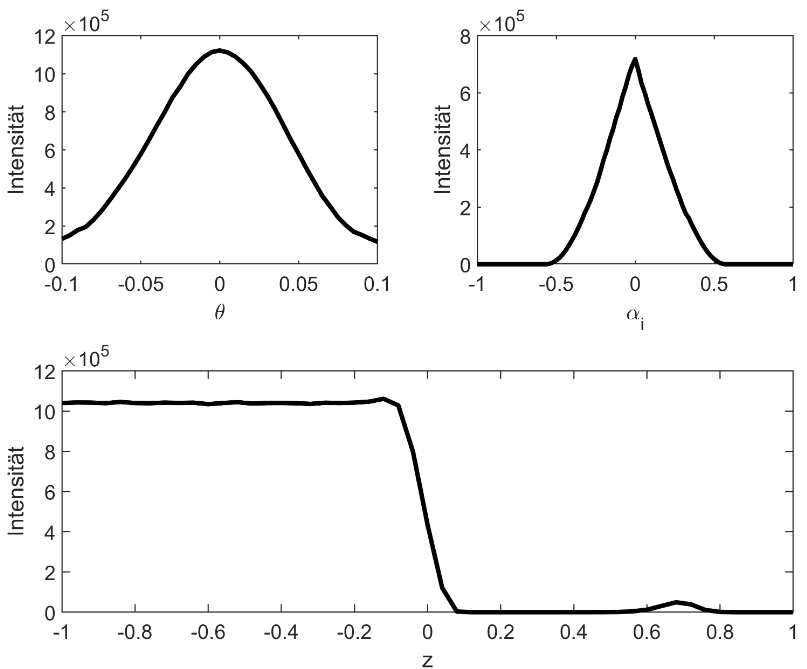
\includegraphics[width=10cm]{übersicht.png}
  \caption{Übersicht, welche Kurvenverläufe bei welchem Scan erwartet werden \cite{skript}.}
  \label{fig:übersicht}
\end{figure}


\subsection{Messung}
Die Messung des Polymerfilms auf dem Silizium-Wafer wird mit einem Reflektivitässcan durchgeführt, bei dem der Winkel $\alpha_i$ zwischen Probe und Strahl gleich dem
Winkel zwischen Probe und Detaktor $\alpha_f$ sind. Als "Scantype" wird am Computer "Omega/2Theta" mit einem Scanbereich von $\SI{0}{\degree}$ bis $\SI{2,5}{\degree}$ gewählt.
Als Schrittweite werden $\SI{0,005}{\degree}$ mit einer Messzeit von $\SI{5}{\s}$ pro Messpunkt gewählt.

Die gemessene Intensität besitzt auch einen gewissen Anteil an gestreuter Intensität. Diese kann durch einen "Diffusen Scan" ermittelt werden, welcher im Anschluss durchgeführt wird.
Dazu wird der Detektorwinkel um $\SI{0,1}{\degree}$ gegenüber dem Einfallswinkel verschoben, während alle anderen Parameter nicht verändert werden.
